\chapter{Continuum mechanics in different frames of reference}
Matter is made up of small building blocks called atoms, that are separated by vacuum, and the fundamental laws at this small scale are described using quantum mechanics. The associated characteristic length scale far smaller than most things of interest at a a macroscopic level. Since it has been observed that the characteristic behavior is statistically uniform, it is reasonable to assume the matter can be mathematically described, and modeled, as a continuum. This allows for a mathematical description at the macroscopic level using Newtonian physical laws to model fluids and solids. The Newtonian laws are generally expressed in one out of two frames of reference, Lagrangian or Eulerian, depending on the physical problem. \newline

To exemplify the differences between these frameworks, one can imagine a river running down a mountain.	
In the Eulerian framework we observe an object following the flow, standing besides the river. We are not necessarily interested in each fluid particle or the history of it, but only how the fluid acts as a whole flowing down the river. The Eulerian framework is especially advantageous to describe fluid mechanics.\newline

A Lagrangian description of solid mechanics is particularly beneficial, as one is generally interested in where the solid particles are in relation to each other and the particles initial spatial state.  
This is best exemplified with a deflecting beam attached to a wall. The more force applied to the beam the more it will deflect, relative to its historical stress free configuration. As described later this frame of reference is generally beneficial to describe stress and strain for solid mechanical problems.\newline

\begin{figure}[H]
\label{pic:E_L}
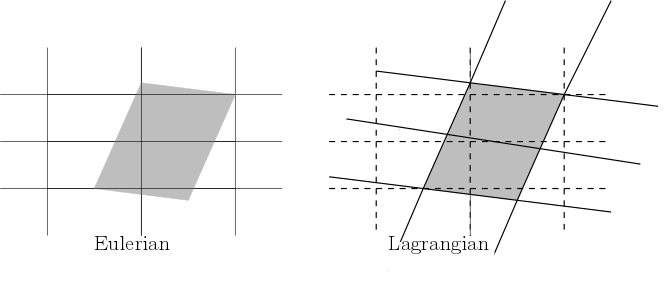
\includegraphics[scale=0.50]{./Continuum_mechanics/E_L.png}
\caption{Comparison between the Eulerian and the Lagrangian description, the lines represent the grid and the gray represents the matter.}
\end{figure}

The goal of this chapter is to briefly introduce convervation of linear momentum for a fluid and a solid, respectively together with the respective boundary conditions. A derivation and a more detailed description of the Lagrangian framework and the stress and strain relations are covered in the appendix A1.

\section{Conservation of mass and momentum for solid matter}
With matter assumed continuous, fundamental physical laws like conservation of mass and conservation of momentum can be applied to derive a differential equation describing the motions of a solid. Information about the particular material of a solid is added through constitutive relations.
The differential solid equation will be stated in the Lagrangian reference system \cite{Holzapfel2000}, in the solid domain $\mathcal{S}$ as:
\begin{equation}\label{eq:Solid}
\rho_s \frac{\partial \bold{d}^2}{\partial t^2} = \nabla \cdot ( P ) + \rho_s f  \hspace{4mm} in \hspace{2mm} \mathcal{S}
\end{equation}
written in terms of the deformation $\bold{d}$, of the solid.
P is the first Piola-Kirchhoff stress tensor, its derivation is included in the appendix A1 for the sake of completeness.
Body forces are denoted as $f$, and are forces that originate outside the body and act on the mass of the body e.g. gravitational force. $\rho_s$ is the solid density, and $\frac{\partial}{\partial t^2}$ is the second time derivative. 

\begin{comment}
\subsection*{Locking}
The problem og shear locking can happen FEM computations with certain elements. 
[mek4250 Kent] - Locking occurs if  $ \lambda >> \nu $ that is, the material is nearly incompressible. The reason is that all the elements discussed in this course are poor at approximating the divergence. Locking refers to the case where the displacement is to small because the divergence term essentially lock the displacement. It is a numerical artifact not a physical feature. [Verbatum]
\end{comment}

\section{Fluid equations}
The Navier-Stokes equations are derived using principles of mass and momentum conservation. These equations describes the velocity and pressure in a given fluid continuum. They are here written in the time domain $\mathcal{F}$:
\begin{align}
\label{eq:NS}
\rho\frac{\partial u}{\partial t} + \rho u \cdot \nabla u &= \nabla \cdot \sigma_f + f \\
\nabla \cdot u &= 0
\end{align}
where $u$ is the fluid velocity, $p$ is the fluid pressure$, \rho$ stands for constant density, f is body force and $ \sigma_f = \mu_f (\nabla u + \nabla u^T)  - pI$ \\
We will only compute incompressible fluids. \\
There does not yet exist an analytical solutions to the N-S equations, only simplified problems can be solved \cite{White2000}. But this does not stop us from discretizing and solving them numerically. \\
Before these equations can be solved we need to impose boundary conditions.
\subsection*{Boundary conditions}
On the Dirichlet boundary $ \partial \mathcal{F}_D$ we impose a given value. This can be initial conditions or set to zero as on walls with "no slip" condition. These conditions needs to be defined for both $u$ and $p$
$$  u = u_0 \text{   on   } \partial \mathcal{F}_D  $$
$$  p = p_0 \text{   on   } \partial \mathcal{F}_D  $$
The forces on the boundaries need to equal an eventual external force $ \bold{f}$
$$ \sigma \cdot \bold{n} = f \text{   on   } \partial \mathcal{F}_N    $$








\section{Fluid and Structure Boundary conditions}
To complete the fluid and solid equations, boundary conditions need to be imposed. The fluid flows and the solid moves within the boundaries noted as $ \partial\mathcal{F}$ and $ \partial \mathcal{S}$ respectively. 

On the Dirichlet boundary, $ \partial \mathcal{F}_D$ and $ \partial \mathcal{S}_D$, we impose a given value. Dirichlet conditions can be initial conditions or set values, such as zero on the fluid boundary for a "no slip" condition. The Dirichlet conditions are defined for $\bold{u}$ and $p$ :
\begin{align}
\bold{u} =& u_0 \text{   on   } \partial \mathcal{F}_D  \\
p =& p_0 \text{   on   } \partial \mathcal{F}_D  \\
\bold{d} =& d_0 \text{ on   } \partial \mathcal{S}_D  \\
\bold{w}(\textbf{X},t)_0 =& \frac{\partial \bold{d}(t=0)}{\partial t} \text{   on   } \partial \mathcal{S}_D   
\end{align}
The forces on the boundaries equal a possible external force $ \bold{f}$. These are are enforced on the Neumann boundaries $\partial \mathcal{F}_N$ and  $\partial \mathcal{S}_N$ :
\begin{align}
\sigma \cdot \bold{n} &= f \text{   on   } \partial \mathcal{F}_N \\   
P\cdot \bold{n} &= f \text{   on   } \partial \mathcal{S}_N    
\end{align}



\begin{comment}
Let $\Omega \in \mathbb{R}^d $ for $d \in \{1,2\}$, be a bounded domain with boundary $ \partial \Omega$. The domain is made up of of two sub domains $ \mathcal{F} $ for the fluid domain, and $\mathcal{S}$ for the solid. The interface between the domains are denoted by $ \Sigma = \mathcal{F} \cap \mathcal{S} $. The reference or initial is denoted by $ \hat{\Sigma} = \hat{\mathcal{F}} \cap \hat{\mathcal{S}}  $ 
\end{comment}

